\documentclass{article}
\usepackage{pgf}
\usepackage{pgfpages}
\usepackage{tikz} % titlepage border
\usetikzlibrary{calc} % titlepage border
\usepackage{niceframe}
\usepackage{graphicx}
\usepackage{textcomp}
\usepackage{fancyhdr}
\usepackage{minitoc}
\usepackage{hyperref}
\usepackage{multicol}
\usepackage{sectsty}
\usepackage{adjustbox}%used for correct positioning of tables
\usepackage{titletoc}
\usepackage{float}


\sectionfont{\fontsize{20}{5}\selectfont}
\subsectionfont{\fontsize{15}{5}\selectfont}
\subsubsectionfont{\fontsize{12}{5}\selectfont}
\usepackage[a4paper, total={6in, 8in}]{geometry}
\newcommand\tab[1][0.5cm]{\hspace*{#1}}

%TitlePage

\begin{document}
\begin{titlepage}
   \begin{tikzpicture}[remember picture,overlay,inner sep=0,outer sep=0]
     \draw[blue!70!black,line width=4pt] ([xshift=-1.5cm,yshift=-2cm]current page.north east) coordinate (A)--([xshift=1.5cm,yshift=-2cm]current page.north west) coordinate(B)--([xshift=1.5cm,yshift=2cm]current page.south west) coordinate (C)--([xshift=-1.5cm,yshift=2cm]current page.south east) coordinate(D)--cycle;

     \draw ([yshift=0.5cm,xshift=-0.5cm]A)-- ([yshift=0.5cm,xshift=0.5cm]B)--
     ([yshift=-0.5cm,xshift=0.5cm]B) --([yshift=-0.5cm,xshift=-0.5cm]B)--([yshift=0.5cm,xshift=-0.5cm]C)--([yshift=0.5cm,xshift=0.5cm]C)--([yshift=-0.5cm,xshift=0.5cm]C)-- ([yshift=-0.5cm,xshift=-0.5cm]D)--([yshift=0.5cm,xshift=-0.5cm]D)--([yshift=0.5cm,xshift=0.5cm]D)--([yshift=-0.5cm,xshift=0.5cm]A)--([yshift=-0.5cm,xshift=-0.5cm]A)--([yshift=0.5cm,xshift=-0.5cm]A);


     \draw ([yshift=-0.3cm,xshift=0.3cm]A)-- ([yshift=-0.3cm,xshift=-0.3cm]B)--
     ([yshift=0.3cm,xshift=-0.3cm]B) --([yshift=0.3cm,xshift=0.3cm]B)--([yshift=-0.3cm,xshift=0.3cm]C)--([yshift=-0.3cm,xshift=-0.3cm]C)--([yshift=0.3cm,xshift=-0.3cm]C)-- ([yshift=0.3cm,xshift=0.3cm]D)--([yshift=-0.3cm,xshift=0.3cm]D)--([yshift=-0.3cm,xshift=-0.3cm]D)--([yshift=0.3cm,xshift=-0.3cm]A)--([yshift=0.3cm,xshift=0.3cm]A)--([yshift=-0.3cm,xshift=0.3cm]A);

   \end{tikzpicture}



\centerline{\LARGE{\textbf{University of Science}}}
\bigskip
\centerline{\large{Viet Nam National University Ho Chi Minh}}

\centerline{\Large{--------------------------------------}}

\bigskip

\centerline{
\includegraphics[width=40mm]{logo.jpg}}

\centerline{\niceframe[14cm]
{
\begin{center}
\LARGE{\textbf{ASSIGNMENT REPORT}}
\end{center}
}}

\bigskip
\bigskip

\centerline{\LARGE{\textbf{COMPUTER SYSTEM}}}
\raggedright
\bigskip
\bigskip

\LARGE{Tutors:}
Thai Hung Van\\
\bigskip
\LARGE{Members:}
\bigskip

21127158 - Lê Hoàng Sang\\
21127511 - Nguyễn Quốc Huy\\
\bigskip
\LARGE{Class: 21CLC02}

\end{titlepage}

\pagestyle{fancy}
\fancyhf{}
\addtolength{\topmargin}{-0.70894pt}
\setlength{\headheight}{12.70894pt}

\lhead{\textbf{FIT-HCMUS}}
\rhead{\textbf{LAB 3: SORTING}}
\rfoot{\textbf{\thepage}}



\tableofcontents

\pagebreak

\section{Information}

\subsection{Assignment content}
\Large{Report the summary of the processor architecture and organization.\\
$=>$ We choose Intel Core™ i9-12900K Processor}

\subsection{Planner}
\Large{
Our work assignments are the following:
\begin{itemize}
    \item 21127158 - Lê Hoàng Sang: 
    \item 21127511 - Nguyễn Quốc Huy:
\end{itemize}
}
\pagebreak


\section{Processor's Introduction}

\begin{tabular}{|c|c|}
\hline
Criteria                           & abc  \\ 
\hline                                                                                                                                                                                                                                                                                                                                                                         \\ \hline
Resulting statics                  & abc  \\ 
\hline
Resulting statics                  & abc  \\ 
\hline
Resulting statics                  & abc  \\ 
\hline
Resulting statics                  & abc  \\ 
\hline


\end{tabular}



\pagebreak


\bigskip

\section{Experimental results and comments}

\subsection{Experimental results}
\subsubsection{Sorted data (in ascending order)}
\begin{table}[H]
\begin{adjustbox}{width=\columnwidth,center}
\begin{tabular}{|l|rrrrrrrrrrrr|}
\hline
                                   & \multicolumn{12}{c|}{Sorted data (in ascending order)}                                                                                                                                                                                                                                                                                                                                                                             \\ \hline
Data size                          & \multicolumn{2}{c|}{10000}                                          & \multicolumn{2}{c|}{30000}                                          & \multicolumn{2}{c|}{50000}                                          & \multicolumn{2}{c|}{100000}                                         & \multicolumn{2}{c|}{300000}                                          & \multicolumn{2}{c|}{500000}                                         \\ \hline
Resulting statics                  & \multicolumn{1}{l|}{Running time} & \multicolumn{1}{l|}{Comparison} & \multicolumn{1}{l|}{Running time} & \multicolumn{1}{l|}{Comparison} & \multicolumn{1}{l|}{Running time} & \multicolumn{1}{l|}{Comparison} & \multicolumn{1}{l|}{Running time} & \multicolumn{1}{l|}{Comparison} & \multicolumn{1}{l|}{Running time} & \multicolumn{1}{l|}{Comparison}  & \multicolumn{1}{l|}{Running time} & \multicolumn{1}{l|}{Comparison} \\ \hline
Selection Sort                     & \multicolumn{1}{r|}{119}          & \multicolumn{1}{r|}{99999999}   & \multicolumn{1}{r|}{1068}         & \multicolumn{1}{r|}{899999999}  & \multicolumn{1}{r|}{2944}         & \multicolumn{1}{r|}{2499999999} & \multicolumn{1}{r|}{11731}        & \multicolumn{1}{r|}{9999999999} & \multicolumn{1}{r|}{105411}       & \multicolumn{1}{r|}{89999999999} & \multicolumn{1}{r|}{292593}       & 249999999999                    \\ \hline
Insertion Sort                     & \multicolumn{1}{r|}{0}            & \multicolumn{1}{r|}{9999}       & \multicolumn{1}{r|}{0}            & \multicolumn{1}{r|}{29999}      & \multicolumn{1}{r|}{0}            & \multicolumn{1}{r|}{49999}      & \multicolumn{1}{r|}{0}            & \multicolumn{1}{r|}{99999}      & \multicolumn{1}{r|}{1}            & \multicolumn{1}{r|}{299999}      & \multicolumn{1}{r|}{2}            & 499999                          \\ \hline
Bubble Sort                        & \multicolumn{1}{r|}{127}          & \multicolumn{1}{r|}{99999999}   & \multicolumn{1}{r|}{1139}         & \multicolumn{1}{r|}{899999999}  & \multicolumn{1}{r|}{3163}         & \multicolumn{1}{r|}{2499999999} & \multicolumn{1}{r|}{12572}        & \multicolumn{1}{r|}{9999999999} & \multicolumn{1}{r|}{113939}       & \multicolumn{1}{r|}{89999999999} & \multicolumn{1}{r|}{315823}       & 249999999999                    \\ \hline
Heap Sort                          & \multicolumn{1}{r|}{2}            & \multicolumn{1}{r|}{504005}     & \multicolumn{1}{r|}{9}            & \multicolumn{1}{r|}{1697716}    & \multicolumn{1}{r|}{16}           & \multicolumn{1}{r|}{22985913}   & \multicolumn{1}{r|}{34}           & \multicolumn{1}{r|}{6375398}    & \multicolumn{1}{r|}{113}          & \multicolumn{1}{r|}{21011202}    & \multicolumn{1}{r|}{196}          & 36433362                        \\ \hline
Merge Sort                         & \multicolumn{1}{r|}{6}            & \multicolumn{1}{r|}{506652}     & \multicolumn{1}{r|}{20}           & \multicolumn{1}{r|}{1694748}    & \multicolumn{1}{r|}{34}           & \multicolumn{1}{r|}{2947020}    & \multicolumn{1}{r|}{69}           & \multicolumn{1}{r|}{6244044}    & \multicolumn{1}{r|}{213}          & \multicolumn{1}{r|}{20367948}    & \multicolumn{1}{r|}{380}          & 35438188                        \\ \hline
Quick Sort & \multicolumn{1}{r|}{1}            & \multicolumn{1}{r|}{163613}     & \multicolumn{1}{r|}{2}            & \multicolumn{1}{r|}{537229}     & \multicolumn{1}{r|}{3}            & \multicolumn{1}{r|}{934461}     & \multicolumn{1}{r|}{7}            & \multicolumn{1}{r|}{1968925}    & \multicolumn{1}{r|}{21}           & \multicolumn{1}{r|}{6375709}     & \multicolumn{1}{r|}{35}           & 10975709                        \\ \hline
Radix Sort                         & \multicolumn{1}{r|}{2}            & \multicolumn{1}{r|}{140038}     & \multicolumn{1}{r|}{7}            & \multicolumn{1}{r|}{510048}     & \multicolumn{1}{r|}{13}           & \multicolumn{1}{r|}{850048}     & \multicolumn{1}{r|}{26}           & \multicolumn{1}{r|}{1700048}    & \multicolumn{1}{r|}{93}           & \multicolumn{1}{r|}{6000058}     & \multicolumn{1}{r|}{161}          & 10000058                        \\ \hline
Shaker Sort                        & \multicolumn{1}{r|}{0}            & \multicolumn{1}{r|}{19999}      & \multicolumn{1}{r|}{0}            & \multicolumn{1}{r|}{59999}      & \multicolumn{1}{r|}{0}            & \multicolumn{1}{r|}{99999}      & \multicolumn{1}{r|}{0}            & \multicolumn{1}{r|}{199999}     & \multicolumn{1}{r|}{1}            & \multicolumn{1}{r|}{599999}      & \multicolumn{1}{r|}{1}            & 999999                          \\ \hline
Shell Sort                         & \multicolumn{1}{r|}{0}            & \multicolumn{1}{r|}{120018}     & \multicolumn{1}{r|}{1}            & \multicolumn{1}{r|}{390021}     & \multicolumn{1}{r|}{2}            & \multicolumn{1}{r|}{700021}     & \multicolumn{1}{r|}{4}            & \multicolumn{1}{r|}{1500022}    & \multicolumn{1}{r|}{14}           & \multicolumn{1}{r|}{5100026}     & \multicolumn{1}{r|}{22}           & 8500025                         \\ \hline
Counting Sort                      & \multicolumn{1}{r|}{0}            & \multicolumn{1}{r|}{89995}      & \multicolumn{1}{r|}{0}            & \multicolumn{1}{r|}{269995}     & \multicolumn{1}{r|}{1}            & \multicolumn{1}{r|}{449995}     & \multicolumn{1}{r|}{2}            & \multicolumn{1}{r|}{899995}     & \multicolumn{1}{r|}{8}            & \multicolumn{1}{r|}{2699995}     & \multicolumn{1}{r|}{15}           & 4499995                         \\ \hline
Flash Sort                         & \multicolumn{1}{r|}{0}            & \multicolumn{1}{r|}{20999}      & \multicolumn{1}{r|}{1}            & \multicolumn{1}{r|}{62999}      & \multicolumn{1}{r|}{2}            & \multicolumn{1}{r|}{104999}     & \multicolumn{1}{r|}{4}            & \multicolumn{1}{r|}{209999}     & \multicolumn{1}{r|}{12}           & \multicolumn{1}{r|}{629999}      & \multicolumn{1}{r|}{21}           & 1049999                         \\ \hline
\end{tabular}
\end{adjustbox}
\end{table}

\begin{figure}[H]
% 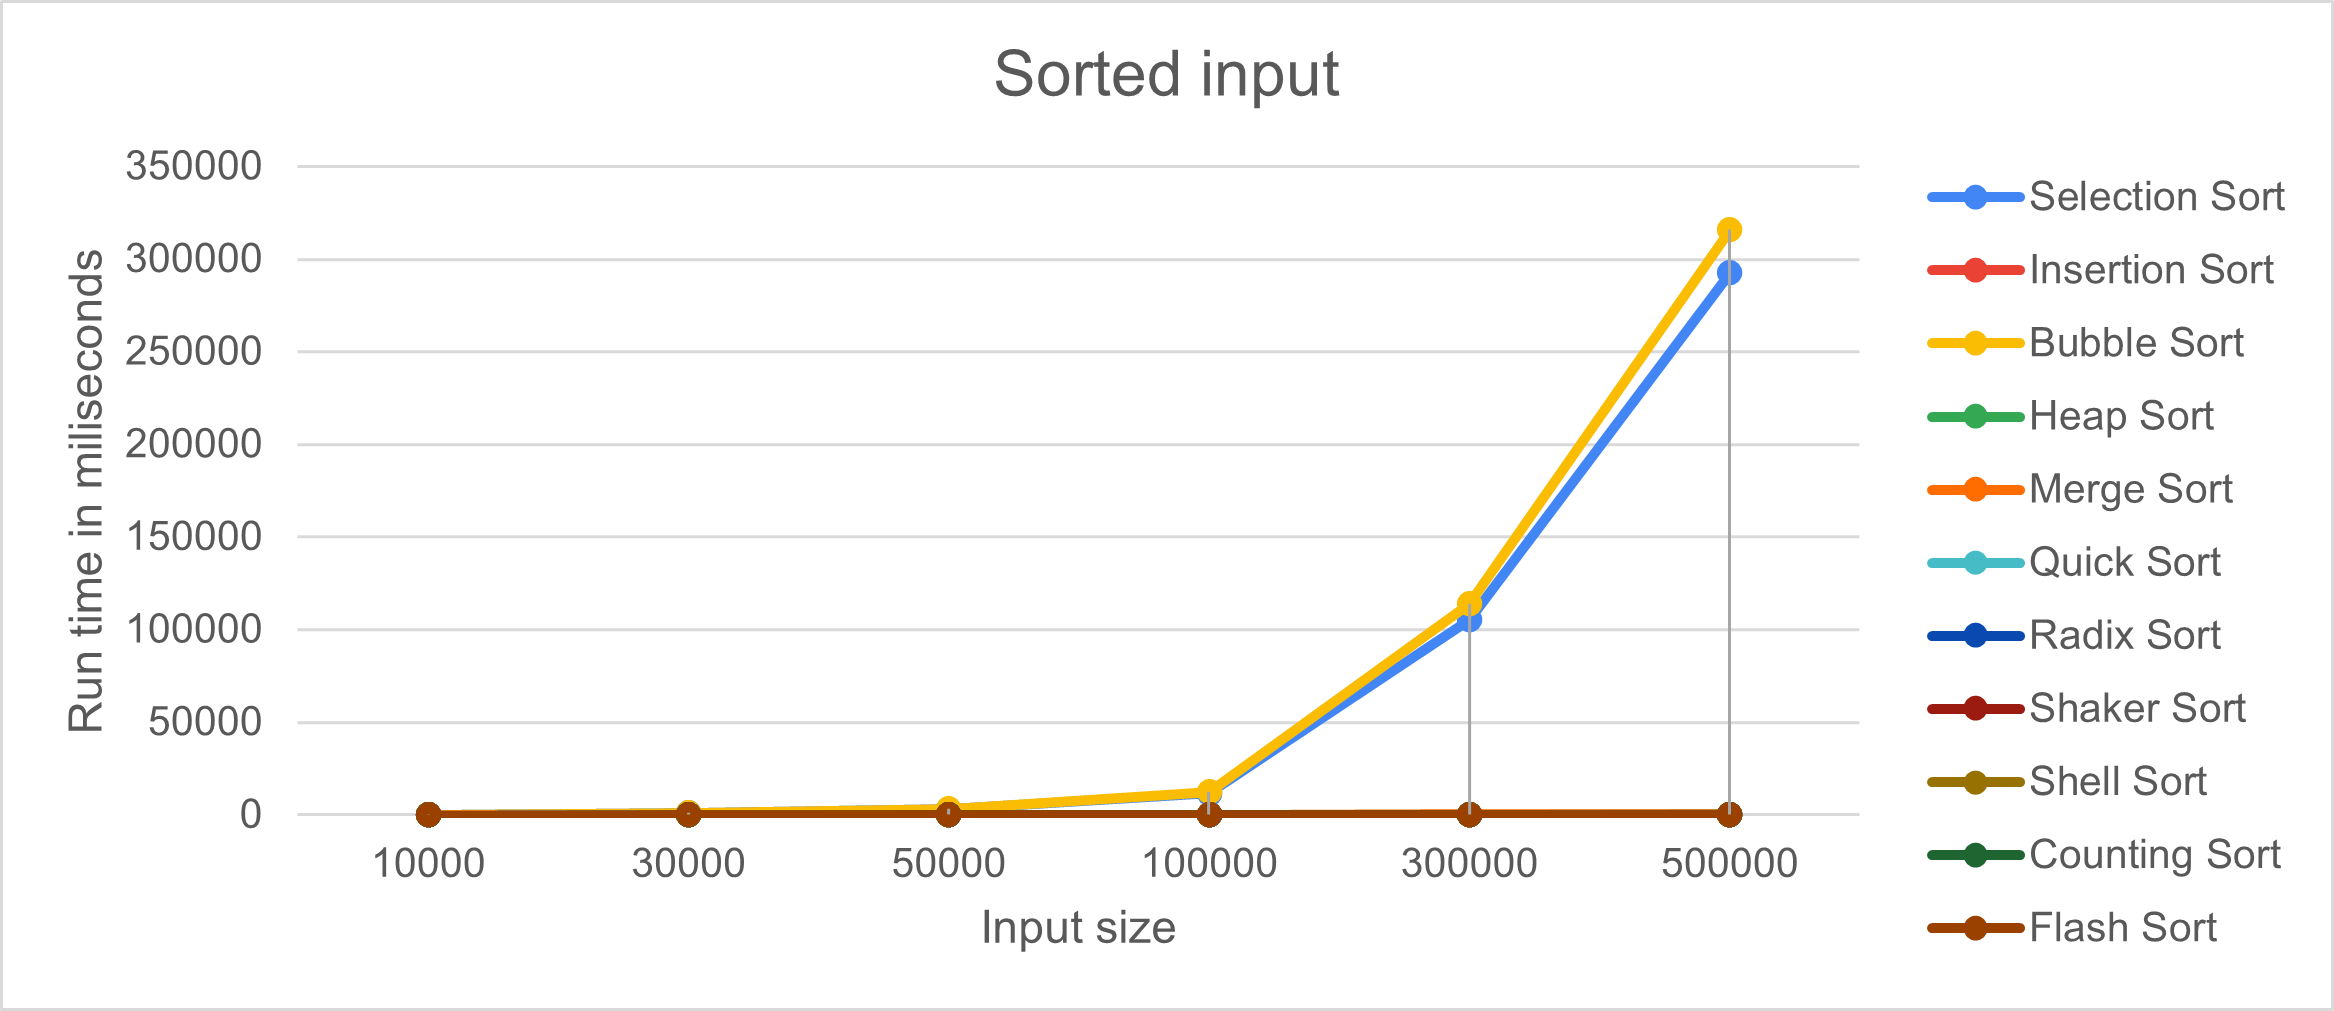
\includegraphics[scale = 0.8]{SortedLines.png}
\caption{ A line graph for visualizing the algorithms’ running times on sorted data.}
\centering
\end{figure}

\tab From what we can see, bubble sort and selection sort take the most amount of time out of all other algorithms when we gradually increases the size of the input data. The time it takes increase exponentially. This is due to the nature of these two sorting algorithms still trying to sort the input while the input itself is already sorted.

\begin{figure}[H]
% 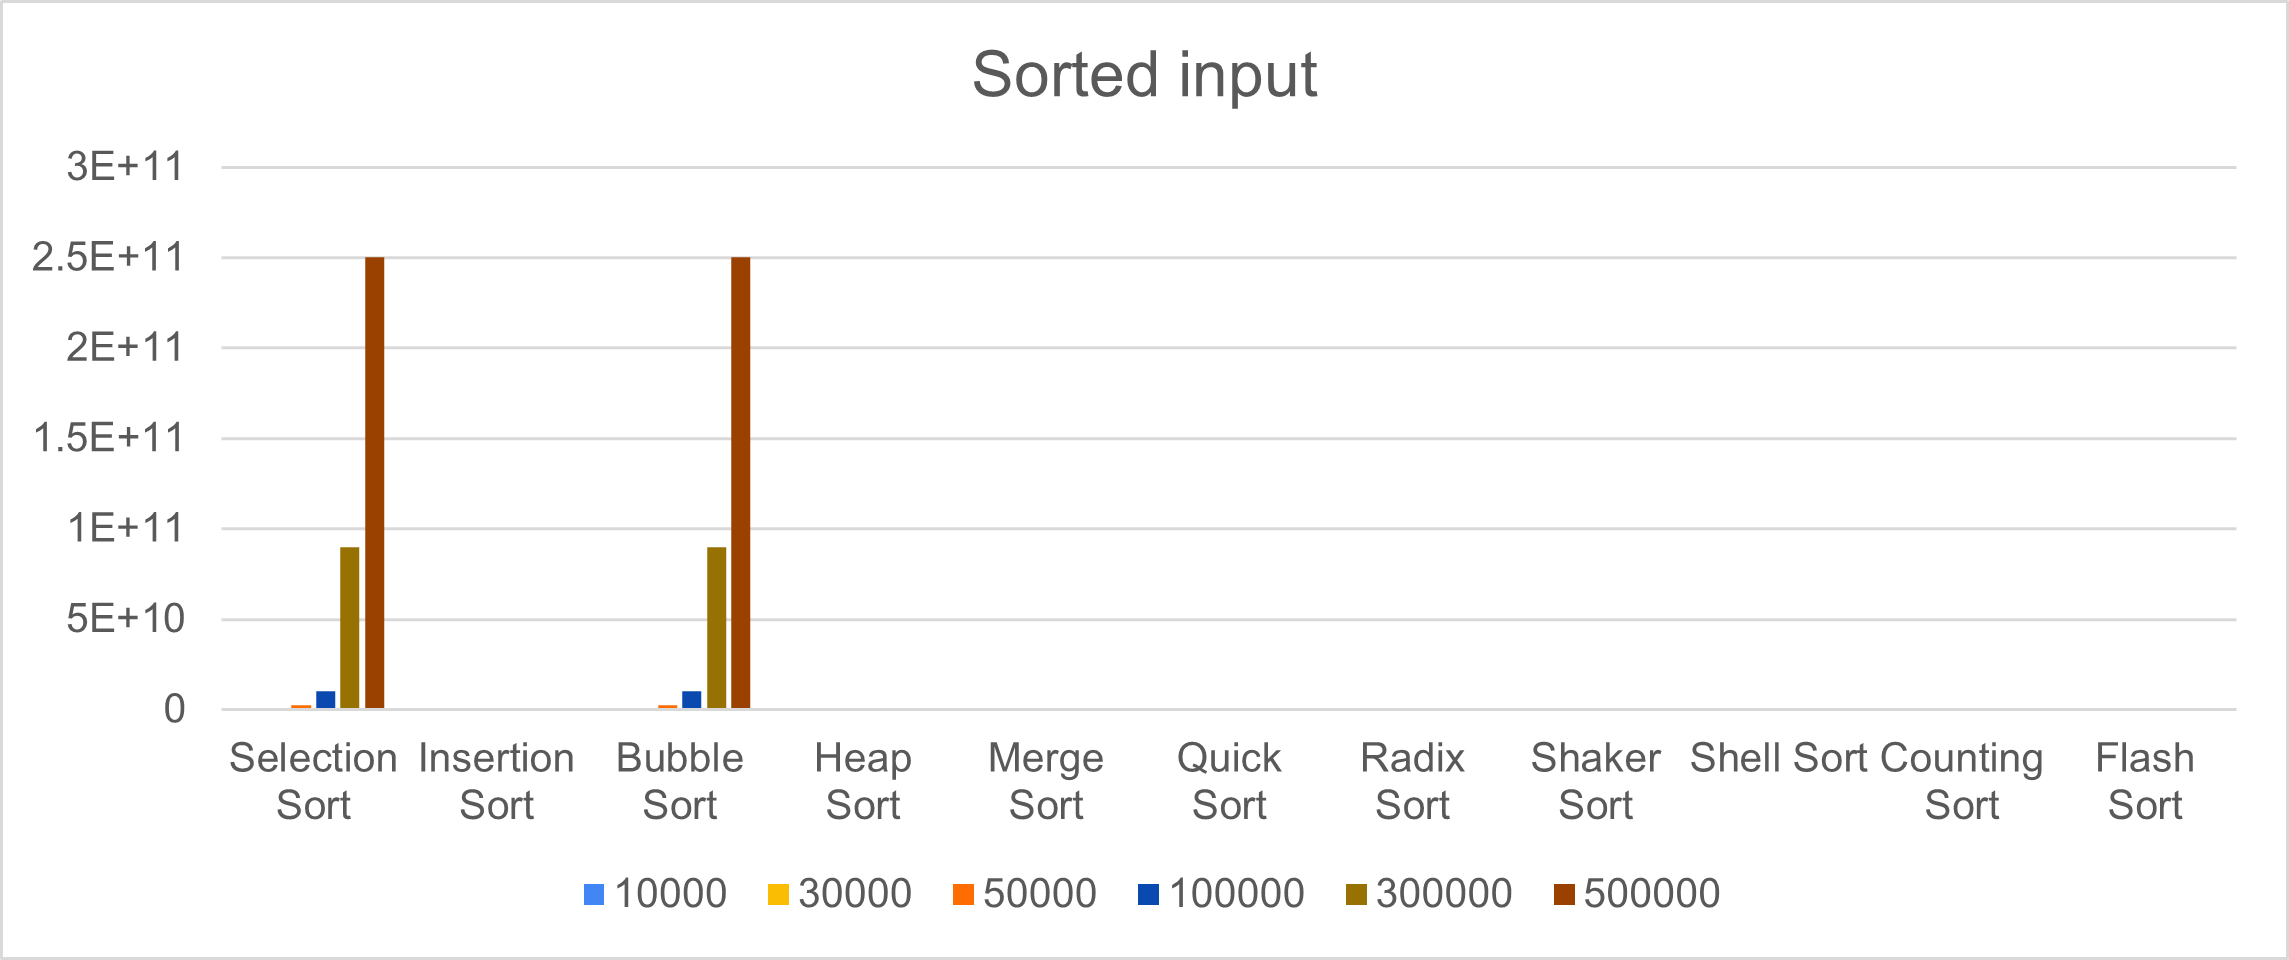
\includegraphics[scale = 0.8]{SortedBar.png}
\caption{A bar graph for visualizing the algorithms’ comparisons on sorted data.}
\centering
\end{figure}

We can see a familiar trend when comparing comparisons, bubble sort and selection sort still take the lead in the most amount of the comparisons. The reason for this is that bubble and selection are comparison-based sorting algorithms, but insertion sort is also comparison-based then why does it take very little comparisons. When the algorithm is already sorted, insertion sort doesn't need to move elements around very much.

\section{References}

\href{https://en.wikipedia.org/wiki/Selection_sort#Complexity}{Information on Selection Sort}\\
\href{https://en.wikipedia.org/wiki/Selection_sort#Complexity}{Selection Sort complexity}\\
\href{https://cs.stackexchange.com/questions/111243/complexity-of-double-selection-sort}{Double Selection Sort complexity}
\href{https://www.geeksforgeeks.org/shellsort/}{Information of Shell Sort}\\
\href{https://en.wikipedia.org/wiki/Shellsort#Description}{Ideas of Shell Sort}\\
\href{https://stackabuse.com/bubble-sort-and-cocktail-shaker-sort-in-javascript/}{Buble Sort and Shaker Sort complexity}\\
\href{https://www.researchgate.net/publication/225806123_A_tight_lower_bound_for_the_worst_case_of_Bottom-Up-Heapsort}{More on bottom up heapsort time complexity}\\
\href{https://www.geeksforgeeks.org/heap-sort/}{Information of heap sort}\\
\href{https://cs.stackexchange.com/questions/11415/how-to-perform-bottom-up-construction-of-heaps}{Idea of Bottom Up Heap Sort}\\
\href{https://www.happycoders.eu/algorithms/heapsort/#Bottom-Up_Heapsort}{Information of Bottom Up Heap Sort}\\
\href{https://en.wikipedia.org/wiki/Binary_tree#Types_of_binary_trees}{Binary Tree}\\
\href{https://www.happycoders.eu/algorithms/heapsort/#Heapsort_Time_Complexity}{Heap Sort complexity}\\
\href{https://en.wikipedia.org/wiki/Heapsort#Variations}{Heap Sort Variants}\\
\href{https://www.geeksforgeeks.org/time-complexities-of-all-sorting-algorithms/}{Time and space complexity for all sorting algorithms and replacing best and worst notation with theta and omega respectively}\\
\href{https://en.wikipedia.org/wiki/Cocktail_shaker_sort#Complexity}{Explanation for line graph of reversed sorted data}\\
\href{https://www.geeksforgeeks.org/quick-sort/}{Information of Quick Sort}\\
\href{https://en.wikipedia.org/wiki/Quicksort#Variants}{Variants of Quick Sort}\\
\href{https://www.geeksforgeeks.org/radix-sort/}{Information of Radix Sort}\\
\href{https://www.simplilearn.com/tutorials/data-structure-tutorial/radix-sort#performance_of_radix_sort_algorithm}{Heap Sort complexity}\\
\href{https://www.growingwiththeweb.com/sorting/radix-sort-lsd/}{Variants of Radix Sort}\\
\href{https://www.javatpoint.com/shell-sort}{Information of Shell Sort}\\
\href{https://en.wikipedia.org/wiki/Counting_sort#Variant_algorithms}{Variants of Counting Sort}\\

\centerline{\Large{~~~~ THE END ~~~~}}
\end{document}